\documentclass{amsart}
\usepackage{tikz}

\title{Strategic games on Xemya}
\author{Tomasz Kowalski}


\begin{document}
\maketitle


\section{Into the oracle's mind}


A curious fact about the oracle is that she is not an oracle at all. She just
happens to know some rudiments of game theory. This being the case, the
oracle sets up a simple model of the situation to guide her through.   

\bigskip

She reasons as follows. Apollonia can either ($A$) accept or ($R$) reject Tysq's
demand. And Tysq can either ($W$) wage war on Apollonia or 
($P$) leave Apollonia at peace. So there are four possible outcomes. 
Here they are as a table
\begin{center}
\begin{tabular}{c|cc}
  & $W$      & $P$ \\
\hline
$A$ & $(M,m)$  & $(K,k)$  \\
$R$ & $(N,n)$  & $(L,\ell)$  
\end{tabular}
\end{center}
where the letters in parentheses stand for the respective payoffs:
upper case for Apollonia, lower case for Tysq. 
Of course, neither the oracle, nor Apollonia's strategists know what the exact payoff
values are, but some reasonable estimates can be worked out. 

If Apollonia refuses, and Tysq attacks, well, 
that will cost Apollonia dearly, say, $N$. If Apollonia accepts, and Tysq attacks
anyway, that will cost Apollonia at least the same plus a blemish
on honour, so $M$ is worse
for Apollonia than $N$, that is, $M < N$. 
Next, if Apollonia accepts and Tysq does not attack, it is certainly a better
outcome than $N$: after all what is stained honour compared to peace. So, $N < K$. 
But now, if Apollonia refuses, and Tysq does not attack---an unlikely, but
not impossible outcome---then this is even better! Peace is kept, honour is
upheld. So, $K < L$. Putting all these together: $M<N<K<L$. For future
reference, let us also introduce the quantities $S = K-M$ and 
$H = N-M$. They can be called, with quite some intuitive appeal 
(check the table!), the \emph{value of peace} and \emph{cost of honour}, respectively. 
Observe that we have $S>H$, so $0<\frac{H}{S} <1$. 
This fraction will be important later. 

Let us now consider Tysq's payoffs. We will steer the simplest course
here, and take Tysq's ultimatum at face value. That is, if Apollonia gives in to
the demand, Tysq will prefer not to attack, which means $m < k$. 
But if Apollonia rejects, then, the demand not being an empty threat, 
Tysq will prefer to attack, so, $n>\ell$. 

\bigskip
Now the oracle faces one more complication. The payoff matrix applies 
to a simultaneous game, but the game she needs to analyse is clearly sequential:
Apollonia moves first, and then, knowing what Apollonia did, Tysq responds. Such games
can be represented as trees. Here is our game:
$$
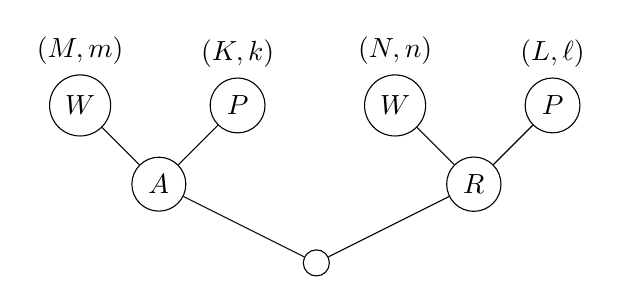
\begin{tikzpicture}
\path node (v0) at (0,0) [circle,draw] {} 
node (v1) at (-2,1) [circle,draw] {$A$} 
node (v2) at (-3,2) [circle,draw,label=above:{$(M,m)$}] {$W$} 
node (v3) at (-1,2) [circle,draw,label=above:{$(K,k)$}] {$P$} 
node (v4) at (1,2) [circle,draw,label=above:{$(N,n)$}] {$W$} 
node (v5) at (3,2) [circle,draw,label=above:{$(L,\ell)$}] {$P$} 
node (v6) at (2,1) [circle,draw] {$R$};
\draw (v0) -- (v1) -- (v2);
\draw (v1) -- (v3);
\draw (v0) -- (v6) -- (v5);
\draw (v6) -- (v4);
\end{tikzpicture}
$$
Apollonia moves first, by either accepting ($A$) or rejecting ($R$) Tysq's
demands. Tysq then responds, by war ($W$) or peace ($P$). At the leaves of the
tree we have the outcomes of following the respective paths. Now, there is 
a neat trick that turns the tree into a game matrix, or to be more precise, 
turns a sequential game into an equivalent simultaneous one. The trick is to
consider Tysq's \emph{conditional strategies}: her strategies as depending of
Apollonia's move\footnote{Games of that kind are sometimes called \emph{meta-games}, for
no good reason.}. Here they are:
\begin{enumerate}
\item $\frac{W}{W}$ -- war regardless of Apollonia's move,
\item $\frac{P}{P}$ -- peace regardless of Apollonia's move,
\item $\frac{W}{P}$ -- war if Apollonia accepts, peace if Apollonia rejects,
\item $\frac{P}{W}$ -- peace if Apollonia accepts, war if Apollonia rejects.
\end{enumerate}
They give rise to the matrix below:
\begin{center}
\begin{tabular}{c|cccc}
  & $\frac{W}{W}$ & $\frac{P}{P}$ & $\frac{W}{P}$ & $\frac{P}{W}$ \\
\hline
$A$ & $(M,m)$     & $(K,k)$       & $(M,m)$       & $(K,k)$  \\
$R$ & $(N,n)$     & $(L,\ell)$    & $(L,\ell)$    & $(N,n)$  
\end{tabular}
\end{center}
with the columns representing Tysq's conditional strategies. 


\bigskip
Having represented the game in the \emph{standard form} above, the oracle 
identifies best responses of each player to the other player's moves. 
\begin{enumerate}
\item If Tysq plays $\frac{W}{W}$, Apollonia's best response is 
$R$, because $M<N$.
\item If Tysq plays $\frac{P}{P}$, Apollonia's best response is
$R$, because $K<L$.
\item If Tysq plays $\frac{W}{P}$, Apollonia's best response is 
$R$, because $M<L$.
\item If Tysq plays $\frac{P}{W}$, Apollonia's best response is
$A$, because $N<K$.
\end{enumerate}
So, Apollonia does not have a move that is always better. In technical terms, 
Apollonia does not have a \emph{dominant} strategy. 

Next, the oracle considers Tysq's best responses.
\begin{enumerate}
\item If Apollonia plays $A$, then Tysq's best response is either 
$\frac{P}{P}$ or $\frac{P}{W}$, as $k>m$.
\item If Apollonia plays $R$, then Tysq's best response is either 
$\frac{W}{W}$ or $\frac{P}{W}$, as $n>\ell$.
\end{enumerate}
So, Tysq does not have a dominant strategy either. However, Tysq has
a \emph{strictly dominated} strategy: a strategy that is never a best response
to anything, namely, $\frac{W}{P}$. Such strategy should never be 
played\footnote{And that is in perfect agreement with intuition, which says
that responding by war to acceptance and by peace to rejection is 
\emph{bloody stupid}, to use another technical term.}, and 
so can be deleted from the matrix. This gives
\begin{center}
\begin{tabular}{c|ccc}
  & $\frac{W}{W}$  & $\frac{P}{P}$  & $\frac{P}{W}$ \\
\hline
$A$ & $(M,m)$      & $(K,k)$        & $(K,k)^\star$  \\
$R$ & $(N,n)^\star$ & $(L,\ell)$     & $(N,n)$  
\end{tabular}
\end{center}
where the two starred outcomes are special. They are special, because
neither player has a strict incentive to move away from a starred outcome, 
if the other player is kept fixed. Indeed, if Apollonia rejects, and Tysq is
playing $\frac{W}{W}$, then moving to $\frac{P}{P}$ would lower Tysq's payoff,
and moving to $\frac{P}{W}$ would leave it unchanged. Similarly,
if Apollonia accepts, and Tysq is playing $\frac{P}{W}$, then
moving to $\frac{P}{P}$ would leave Tysq's payoff unchanged, and 
moving to $\frac{W}{W}$ would lower it. Considering these two outcomes from
Apollonia's point of view, if Tysq plays $\frac{W}{W}$ and Apollonia plays $R$,
then moving to $A$ lowers Apollonia's payoff; if Tysq plays
$\frac{P}{W}$ and Apollonia $A$, then moving to $R$ lowers Apollonia's payoff,
too. Such situations are called \emph{Nash equilibria}. 


\bigskip
The problem with them is they are two, and two is too many. Were there only one,
the game would inevitably finish there, and the recommended strategy 
for each of the players would be the one that leaves them at the Nash
equilibrium. As matters stand, however, it is not so simple. 
Enter probabilities. Let the probability of
Tysq's playing $\frac{W}{W}$ be $p_1$, the probability of
Tysq's playing $\frac{P}{P}$ be $p_2$, and the probability of
Tysq's playing $\frac{P}{W}$ be $p_3$. Of course, Tysq must play
something, so $p_1 + p_2 + p_3 = 1$. Next, the oracle makes a
simplifying assumption. She observes that Tysq's playing the $\frac{P}{P}$
strategy would amount to bluffing: testing Apollonia's resolve, with no real
intention of going to war. This seems unlikely: $p_2$ must be rather low.
How low? She does not know, but to simplify calculations, which
must be rough anyway, she assumes it is negligible. So she can set $p_2 = 0$, and
thus $p_1 = p$ and $p_3 = 1-p$, for some $p\in[0,1]$. The \emph{expected utility} for
Apollonia of playing $A$ is then
$$
EU_A = pM +(1-p)K
$$
For the mathematically challenged: $EU_A$ is Apollonia's payoff if Tysq
plays $\frac{W}{W}$ weighted by the likelihood of Tysq's playing 
$\frac{W}{W}$ plus Apollonia's payoff if Tysq plays
$\frac{P}{W}$ weighted by the likelihood of Tysq's playing 
$\frac{P}{W}$. For even more
mathematically challenged: it is a natural average of the payoffs.
Similarly, Apollonia's expected utility of playing $R$ is 
$$
EU_R = pN +(1-p)N = N
$$
calculated as before but with payoffs from the row $R$. The strategy Apollonia
should choose, according to game-theoretic wisdom, is 
\begin{itemize}
\item $A$ if $EU_A > EU_R$,
\item $R$ if $EU_A < EU_R$,
\item a randomised mix of $A$ and $R$ if $EU_A = EU_R$.
\end{itemize}
Sparing the reader some simple algebra, these translate to
\begin{align*}
A &\quad\text{ if } \frac{H}{S} < 1-p,\\
R &\quad\text{ if } \frac{H}{S} > 1-p,\\
\text{mix} &\quad\text{ if } \frac{H}{S} = 1-p.
\end{align*}
where $S = K-M$ (the value of peace) and $H = N-M$ (the cost of honour). Observe
that the higher the value of $p$ (that is, the probability that Tysq plays
$\frac{W}{W}$), the more reasonable it becomes for Apollonia to play $R$.
But also, the lower the value of $H$ relative to $S$, the more reasonable it
becomes to play $A$. 


\bigskip
Can the oracle say anything at all about the values of $p$, $S$ and $H$? Well,
not on her own. But she can ask---which she does. The first question is about
$p$, and this can be rather direct. The second question, about $\frac{H}{S}$, 
must be asked in a roundabout way if the oracle does not want to
give an introductory lecture on game theory first. 
Translated into our technical terminology the second question is: 
How big is $H$ in comparison to $S$.


\section{A final comment}


For someone familiar with Apollonia's history,
it will come as no surprise that one estimate of $H$ was given by 
none other than Apollonia's Prime Minister at the time. In a famous speech, he
said: 
\begin{quote}
Peace is a valuable and desirable thing. But peace, as almost all affairs of
this world, has its price: high, but assayable. In Apollonia we do not recognise  
the concept of peace at any cost. There is only one thing in lives of
men, peoples and states, which is priceless: this thing is honour.
\end{quote}
Passionate rhetoric nothwithstanding, what this passage says is quite simple:
$H$ is much greater than $S$. Suppose it really is the case that $H>S$. Then, 
$\frac{H}{S} > 1$ and so $\frac{H}{S} > 1-p$ regardless of what $p$ is.
The strategy Apollonia should then rationally choose is $R$: precisely the
strategy she did in fact choose.  However, such dramatically high estimate is by
no means necessary. As we saw, it suffices to have a high estimate of $p$, and
not ridiculously low estimate of $H$.  


\bigskip
Is there a moral to this story? I think there are quite a few, but I leave most
of them to the reader. I wish to state one only: there are games in which it is
not irrational to adopt a strategy that inevitably leads to disastrous
consequences. In plain Apollonian: there are games that cannot be won.


\end{document}


%%% Local Variables:
%%% mode: latex
%%% TeX-master: t
%%% End:
